\chapter{Results}\label{cha:results}

This section will present and discuss the results from our experiments.
The modified SSD model presented in Section~\ref{sec:method-arch} is trained according to the training procedure given in Section~\ref{sec:method-exp-setup}.
Section~\ref{sec:results-baseline} presents the performance of the baseline model. 
The results from experiments pertaining to RQ1 and RQ2 are presented in Section~\ref{sec:results-simplification} and Section~\ref{sec:results-sharpness} respectively.
Unless specified otherwise, all performance metrics given in this section are measured on the test split of the dataset.
For measuring mAP we use an IoU of 0.5 as the acceptance threshold, and follow the interpolation method specified in Equation~\ref{eq:average-precision}

\section{Baseline model}\label{sec:results-baseline}
\begin{figure}[htb]
    \centering
    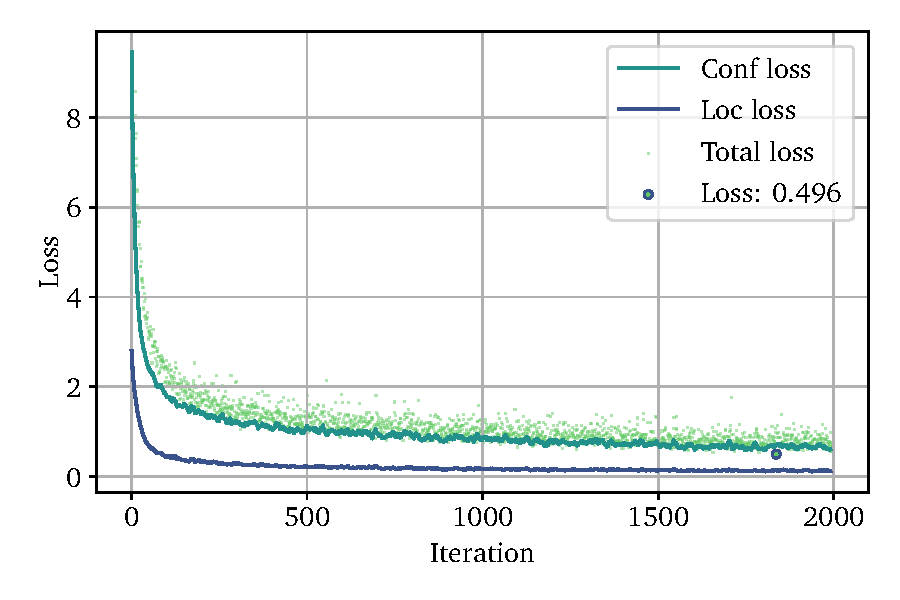
\includegraphics[width=0.7\textwidth]{figs/method/baseline/loss2.pdf}
    \caption[Baseline training procedure]{%
Training procedure for the baseline model over 2000 iterations.
The iterations are given on the horizontal axis are represent one forward-backpropagation run with one mini-batch, while the mini-batch averaged loss is given in the vertical axis.
The raw total loss values are shown with semi-transparent green points.
The solid lines show the moving means for the two individual loss components.
The green line shows the confidence loss component, while the blue line shows the localization loss component.
The mini-batch with the lowest total loss is annotated with a green circle and occurs after the 1800th iteration with a loss of 0.496.
    }\label{fig:method-baseline-loss}
  \end{figure}

We start by presenting the results from training the model in its baseline configuration. 
The training procedure is given in Figure~\ref{fig:method-baseline-loss}.
The stochastic variation in the loss curve is characteristic for mini-batch training. 
We can also see that the confidence loss accounts for most of the total loss throughout the training process.
The components of the loss function (Equation~\ref{eq:loss}) are independent, meaning that their ratio does not indicate a difference in performance at the two different tasks.
We do however observe that the model performs better at localization than classification.
Logically this follows from the realization that the pollen grains are all distinct from the background, but are all quite similar.
The model is therefore able to discriminate between background and pollen with relative ease, but has a harder time classifying species.

\begin{figure}[htb]
    \centering
    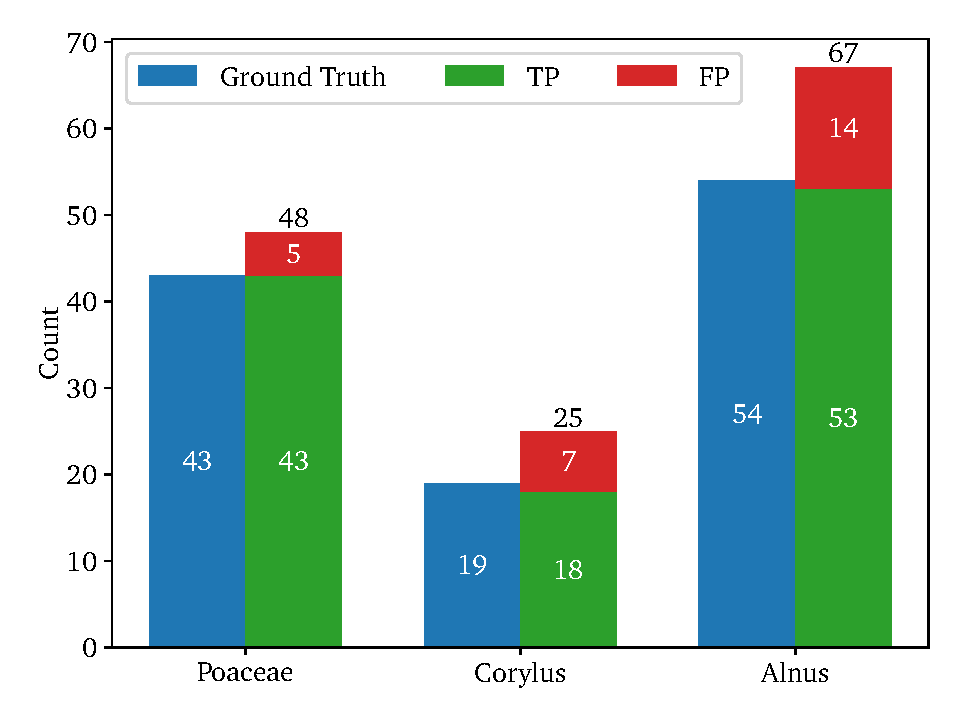
\includegraphics[width=0.7\textwidth]{figs/method/baseline/detections_test.pdf}
    \caption[Detections by type by class for the baseline on the test split] and an \(F_1\) score of \textbf{86.8\%}.
Looking at predictions overall the recall is very high at 99.1\%, while precision is quite a bit lower at 77.2\%.
Figure~\ref{fig:method-baseline-detections} breaks down all the detections made, the main observation is that false positive predictions are the almost singular source of error.
37\% of false positives are miss-localizations, i.e.~an unlabeled entity is identified as a pollen grain.
These entities are either non-pollen particles or pollen grains from unlabeled species.
The remaining 63\% of false positives are miss-classifications, i.e.~the bounding box does correspond to a ground truth, but the class is incorrect.

\begin{figure}[htb]
  \centering
  \begin{subfigure}[t]{0.4\textwidth}
    \centering
    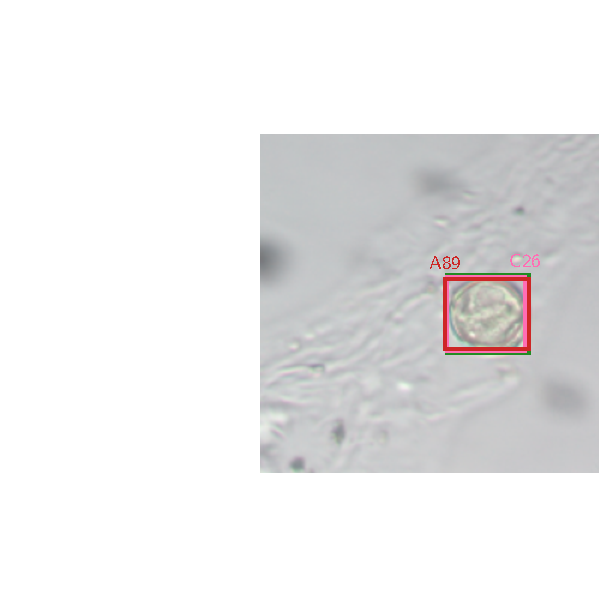
\includegraphics[width=\textwidth]{figs/method/baseline/Snap-408.pdf}
  \end{subfigure}%
  \hspace*{0.04\textwidth}
  \begin{subfigure}[t]{0.4\textwidth}
    \centering
    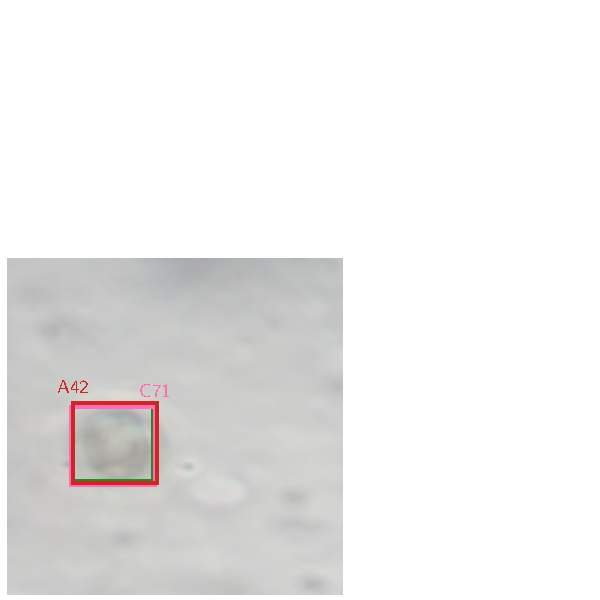
\includegraphics[width=\textwidth]{figs/method/baseline/Snap-028.pdf}
  \end{subfigure}
  \caption[Predictions showing TP overlapped by FP from different class]{Two predictions with GT in \textcolor{nicegreen}{green}, TP in \textcolor{red}{red}, and FP in \textcolor{nicepink}{pink}.
The labels give the first letter of the class and the prediction confidence in the range [0,100].
All TP labels are placed at the NW corner of the bounding box.
The FP labels are placed at the other three corners according to class.
In the left image, a FP box is predicted with a lower confidence than the TP\@.
In the right image, the FP corylus prediction has a higher confidence than the TP alnus prediction.}\label{fig:method-overlapping-predictions}
\end{figure}


%\section{Model simplification}\label{sec:results-simplification}

%\section{Sharpness}\label{sec:results-sharpness}